\section{Transitioning Multi-View OOD Detection using Attention}
\label{sec:propwork-scod}

The expansion of multi-view OOD detection to realistic application environments involves many factors. One critical factor is generalizability across architecture. With the recent advent of Transformers \cite{vaswani2017attention} in ML, a natural evolution of multi-view OOD detection is the incorporation of techniques exploited by Transformer models. Attention, described in Chapter \ref{diss_bkgd}, is a fundamental computational component in Transformer models and a natural complement to multi-view processing. The conceptual foundation of Attention is the ability for sections of images to ``attend'' to, or identify and reinforce the features of, other sections of the image. Applying this concept to the multi-view framework, Attention enables different views to verify and strengthen correlated (i.e. discriminative) features across views while simultaneously dampening irrelevant or noisy (i.e. spurious) features. This positive reinforcement effect improves the extraction of discriminative features, thus benefiting OOD detection.

This section focuses primarily on the architectural improvements towards improved multi-view OOD detection. The data issues described in previous sections (i.e. for MOD and MEO) are not addressed here but in the next chapter (see Chapter \ref{diss_casod}). Instead, this section is an incremental improvement on MOD that introduces and demonstrates the functionality and benefits of Attention in the proposed FgBg multi-view OOD detection domain.

%Attention \cite{} deserves its own introduction, both for its existing impact and for the role it plays in improved multi-view OOD detection. Details for the Attention mechanism and considered component details can be found in Section {\color{red}TODO}. Attention effectively identifies which subsections of the image to attend to with respect to the optimization objective. The delineation of ``self-attention'' refers to the fact that the same input $x$ is used to compute each component ($Q$, $K$, $V$) for attention. Thus the attention mechanism references to and emphasizes components of itself when identifying important features. Cross-attention uniquely considers two inputs and the interaction they have with each other. Given a $Q$ that is computed from a view $x_1$ and $K$, $V$ computed from a view $x_2$), information in $x_1$ is referenced to identify and emphasize relevant feature information in $x_2$. This allows for the model to exploit the information in \emph{multiple inputs} to learn rich, correlated feature information across inputs. These state-of-the-art processing mechanisms enable learning of detailed, informed features conducive to classification, or more relevantly, OOD detection.

The resultant improved method is denoted as %\textbf{S}elective \textbf{C}ross-view \textbf{O}OD \textbf{D}etection (\sysc)
Selective Cross-view OOD Detection (SCOD). SCOD leverages the benefits of Attention mechanisms via cross-attention to improve extraction of discriminative features from both the original image and the foreground-background views. After view selection, the original image features and the selected view features are fused using cross-attention. This replaces the MaxPooling fusion method in MOD. The other components in SCOD are similar to MOD, but the resultant OOD detection performance surpasses that of the naive selection and MaxPooling method in MOD.

\subsection{Proposed Method}
\label{sec:propwork-scod-propmeth}

\begin{figure*}
 \centering
 %\fbox{\rule{0pt}{2in} \rule{0.9\linewidth}{0pt}}
 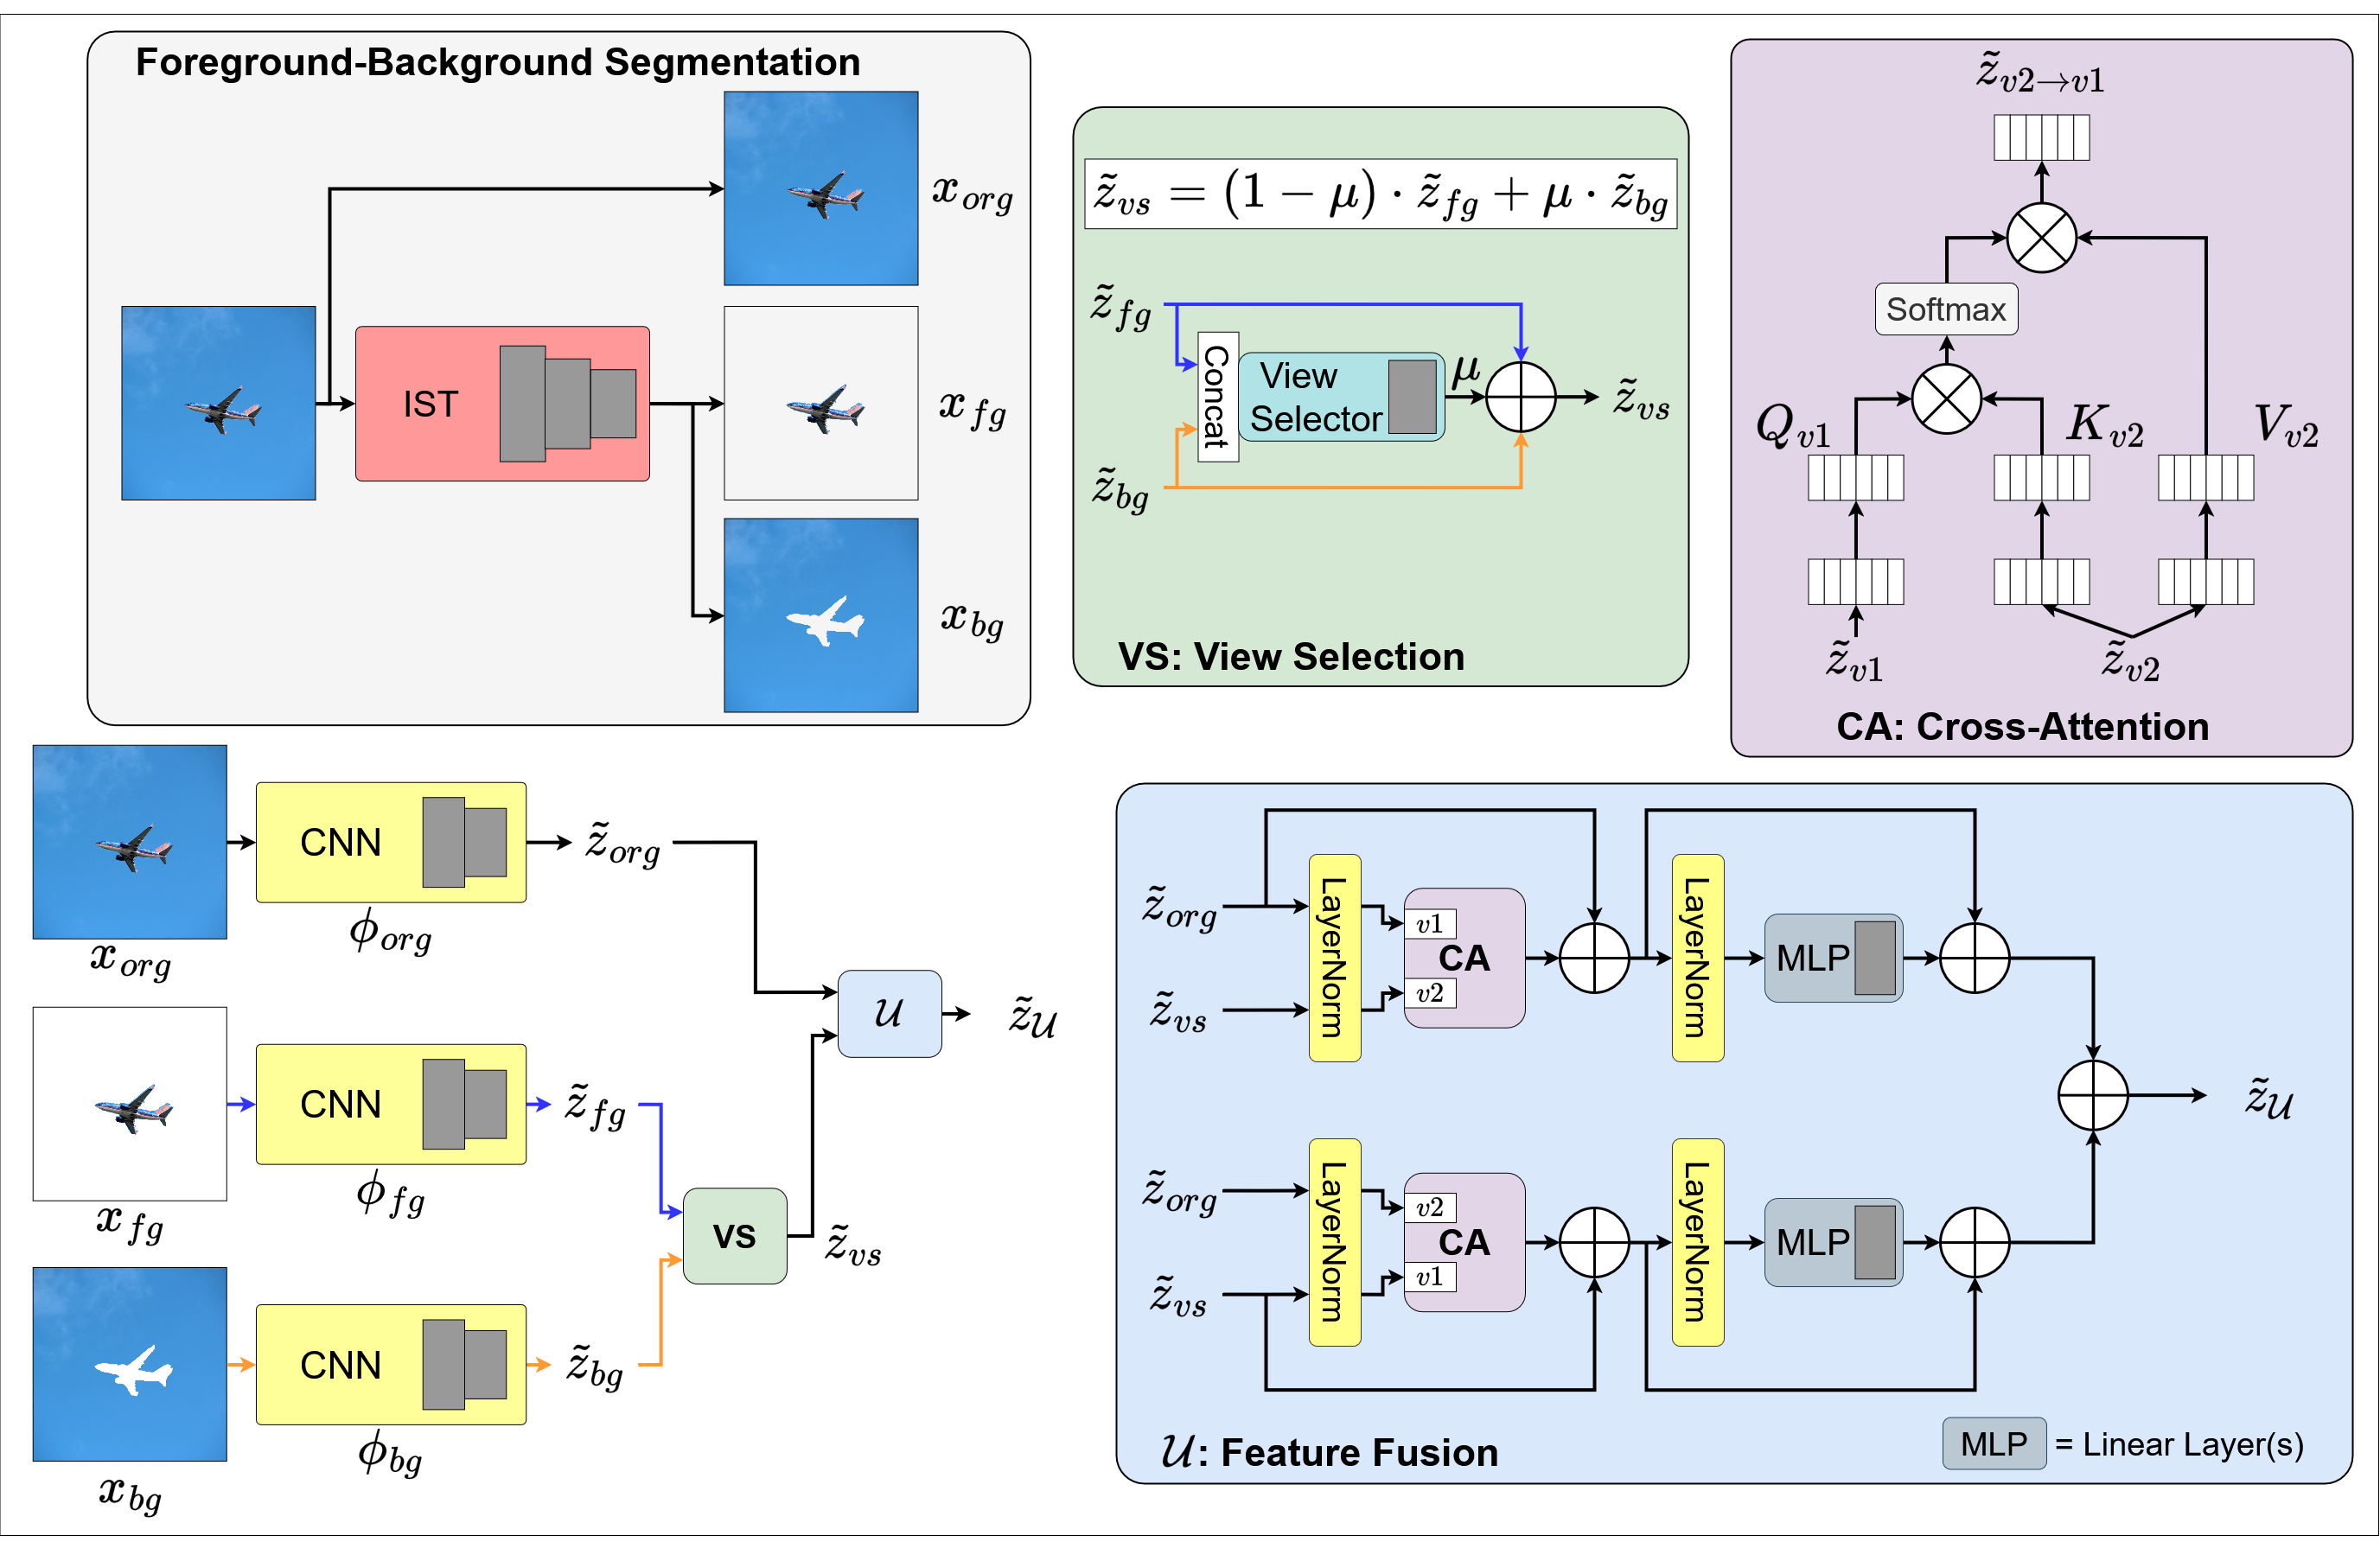
\includegraphics[width=1.\linewidth]{figures/scod_diagram}
  \caption{Model architecture of the proposed \sysc. %Foreground-background segmentation was done on entire datasets during setup. Black lines refer to the original or fused image features. Blue lines refer to foreground image features, orange lines refer to background image features.
  }
\label{fig:propwork-scod-diagram}
\end{figure*}

%\sysb resembles \sysa in that a MVCNN is used for the FgBg multi-view model $f_{MV}$ backbone. Each feature extractor $\phi_v = f_{\theta,v}$ (parameterized by $\theta$) outputs a $d$-dimensional feature vector from input view $x_v$, $\phi_v: \mathcal{X} \mapsto \mathbb{R}^d$. The multi-view feature extractors $\phi_{MV}$ give $Z_{MV} = \{z_{org}, z_{fg}, z_{bg}\}$ with corresponding classification parameters $W_{MV}$ and $b_{MV}$ subsequently outputting $\hat{Y}_{MV} = \{\hat{y}_{org}, \hat{y}_{fg}, \hat{y}_{bg}\}$. The fusion component $\mathcal{U}$ in \sysb differs significantly from \sysa, instead constructing the single-view features, cross-view features, and comprehensive fused feature for ensembling.
The structure of SCOD is similar to that of MOD and MEO. An MVCNN is used as the backbone for the FgBg multi-view model $f_{MV}$, with multi-view feature extractors $\phi_v = f_{\theta,v}$, parameterized by $\theta$, taking as input views $x_v$ and providing as output view features $\tilde{z}_v = \phi_v (x_v)$. Note, however, that in SCOD, view features are extracted \textbf{prior to the average-pooling and flattening operations} (and thus are not vectors). That is, $\phi_v: \mathcal{X} \mapsto \mathbb{R}^{\mathcal{I} \times \mathcal{J} \times \mathcal{K}}$, where $\mathcal{I}$ is the image convolution channel dimension, $\mathcal{J}$ is the image convolution width dimension, and $\mathcal{K}$ is the image convolution height dimension. Feature vectors are computed by applying average-pooling and flattening operations to features, $z_v = flat(\text{AvgPool}(\tilde{z}_v))$, where $flat(\cdot)$ is a matrix-flattening operation converting from $\mathbb{R}^{\mathcal{I} \times 1 \times 1}$ to $\mathbb{R}^{\mathcal{I}}$ and $\text{AvgPool}$ is an average-pooling operation across dimension $\mathcal{J} \times \mathcal{K}$ (collapsing $\mathbb{R}^{\mathcal{I} \times \mathcal{J} \times \mathcal{K}}$ to $\mathbb{R}^{\mathcal{I} \times 1 \times 1}$). For SCOD, $f_{MV}$ outputs multi-view features $\tilde{Z}_{MV} = \{\tilde{z}_{org}, \tilde{z}_{fg}, \tilde{z}_{bg}\}$ and feature vectors $Z_{MV} = \{z_{org}, z_{fg}, z_{bg}\}$. Individual classification parameters $W_{MV}$, $b_{MV}$ take as input $Z_{MV}$ and output prediction logits $\hat{Y}_{MV} = \{\hat{y}_{org}, \hat{y}_{fg}, \hat{y}_{bg}\}$. The fusion component $\mathcal{U}$ for SCOD uses the view selector from MOD but dramatically upgrades the feature fusion computation by introducing the usage of Transformer-inspired \emph{cross-attention} \cite{vaswani2017attention}.

%The diagram in Figure \ref{fig:propwork-mod-diagram} illustrates the high-level operations and flow of information in \sysa. An IST segments an image into a foreground view and a background view. The MVCNN architecture converts the input original image view (\textit{org}), foreground view (\textit{fg}), and background view (\textit{bg}) to view-specific feature vectors $Z_{MV} = \{z_{org}, z_{fg}, z_{bg}\}$. Each feature extractor $\phi_v$ in \sysa is implemented with a ResNet-18 \cite{he2016deep} model. Of note, however, is that the design of \sysa is modular. Any model capable of processing an input image and outputting a feature vector $z_v \in \mathbb{R}^d$ is compatible. The fusion component in \sysa $\mathcal{U}_{\text{\sysa}}$ uses \emph{view selection} to combine information in $Z_{MV}$ into a fused feature vector $z_{\mathcal{U}} = \mathcal{U}_{\text{\sysa}}(Z_{MV})$, $z_{\mathcal{U}} \in \mathbb{R}^d$.
%The flow of information for \sysb is illustrated in Figure \ref{fig:propwork-meo-diagram}. The IST segments the original image view (\textit{org}) into a foreground view (\textit{fg}) and a background view (\textit{bg}). The MVCNN backbone generates features $Z_{MV}$ and logits $\hat{Y}_{MV}$. In \sysb, the fusion component $\mathcal{U}$ is composed of three modules.
The information flow for SCOD is presented in \ref{fig:propwork-scod-diagram} and follows that of MOD closely, with the IST segmenting the original image view (\textit{org}) into foreground (\textit{fg}) and background (\textit{bg}) views, the MVCNN backbone generating features $\tilde{Z}_{MV}$, feature vectors $Z_{MV}$, and logits $\hat{Y}_{MV}$ from the views, and the fusion component $\mathcal{U}_{\text{\sysc}}$ combining view information into fused feature $\tilde{z}_{\mathcal{U}}$. Notably, $\mathcal{U}_{\text{\sysc}}$ differs from MOD in the fusion mechanisms after view selection. Overlapping details are not mentioned in this section and instead should be assumed to mimic those in Section \ref{sec:propwork-mod-propmeth}.

%\textbf{View Selector:} The view selector is implemented using a fully connected layer $f_{\theta}$ that takes the concatenation of average-pooled and flattened foreground and background features $[z_{fg,flat}; z_{bg,flat}] \in \mathbb{R}^{2C}$ as inputs and outputs a view selection weight $s$
%\begin{equation}
%\begin{split}
%    z_{fg,flat} & = flat(\text{AvgPool}(z_{fg})) \in \mathbb{R}^{C} \\
%    z_{bg,flat} & = flat(\text{AvgPool}(z_{bg})) \in \mathbb{R}^{C} \\
%    s & = \sigma (f_{\theta}([z_{fg,flat}; z_{bg,flat}]))
%\end{split}
%\end{equation}
%where $flat(\cdot)$ is a matrix-flattening operation converting from $\mathbb{R}^{C \times 1 \times 1}$ to $\mathbb{R}^{C}$, $\text{AvgPool}$ is an average-pooling operation across dimensions $H \times W$ (collapsing $\mathbb{R}^{C \times H \times W}$ to $\mathbb{R}^{C \times 1 \times 1}$), and $\sigma$ is the sigmoid function.~Note,~the view selector is class-agnostic.~The original view feature $z_{org}$ does not take part in view selection as it contains overall semantic information. We always include it in feature fusion. The view selector features $z_{vs}$ is the sum of $z_{fg}$ and $z_{bg}$ weighted by $s$
%\begin{equation}
%     z_{vs} = (1 - s) \cdot z_{fg} + s \cdot z_{bg}
%\end{equation}
\subsubsection{View Selector}
The view selection operation in SCOD is identical to that in MOD. It takes as input the foreground and background view-specific feature vectors $z_{fg}, z_{bg}$ and produces as output the view selection weight $\mu$. See Section \ref{sec:propwork-mod-propmeth} for details.

%\textbf{Feature Fusion:} The view selection feature $z_{vs}$ contains the ID class-relevant feature information between the foreground and background views. This information is complementary to the feature information in $z_{org}$. %and can identify critical feature information across views useful for identifying ID image classes. 
%Cross-attention allows models to focus on class-relevant discriminative information in images represented across different views via attention weights learned using features from both views \cite{tsai2019multimodal,wang2024mutualformer,lee2024crossformer}. As such, we use a cross-attention architecture to learn these cross-view complementary features from the original view and the selected view.%, inspired by previous work using cross-attention techniques \cite{tsai2019multimodal,wang2024mutualformer,lee2024crossformer}.} %In our proposed cross-attention feature fusion module, we introduce a \textit{cross-view correlation} operation that explicitly encourages alignment between the original feature and view selection feature for greater informative transfer and discriminative feature learning.
%
%The cross-attention feature fusion module receives as input $z_{org}$ and $z_{vs}$. Both features are reshaped from $\mathbb{R}^{C \times H \times W}$ to $\mathbb{R}^{T \times d}$. $T$ is the sequence length resulting from dividing the spatial dimensions into tokens and appending a class token, i.e. $T = 1 + H \times W$. $d$ is the channel information of the feature, i.e. $d = C$. We also add position encodings to $z_{org}$ and $z_{vs}$.
%
%The fusion module is composed of two branches, one a reflection of the other. Without loss of generality, we represent the inputs to a branch as $z_{v1}$ and $z_{v2}$. A branch takes $z_{v1}$ and $z_{v2}$ and extracts queries $Q = FF_{Q}(LN(z_{v1})) \in \mathbb{R}^{T_{v1} \times d_{k}}$ from $z_{v1} \in \mathbb{R}^{T_{v1} \times d_{v1}}$ using feed-forward layer $FF_{Q}$ ($LN$ is the LayerNorm operation), and keys $K = FF_{K}(LN(z_{v2})) \in \mathbb{R}^{T_{v1} \times d_{k}}$ and values $V = FF_{V}(LN(z_{v2})) \in \mathbb{R}^{T_{v1} \times d_{w}}$ from $z_{v2}$ using feed-forward layers $FF_{K}$ and $FF_{V}$. These queries, keys, and values are then used to generate the cross-attention features $z_{v2 \rightarrow v1}$
%%The cross-attention feature fusion module receives as input the original view convolutional features $z_{org} \in \mathbb{R}^{T_{org} \times d_{org}}$ from the penultimate layer of the original view feature extractor $\phi_{org}$ and the view selection features $z_{vs} \in \mathbb{R}^{T_{vs} \times d_{vs}}$. $T_{(\cdot)}$ is the sequence length and $d_{(\cdot)}$ is the feature dimension. (Note that we follow the Transformer format and append a class token to the convolutional dimension i.e. $T = 1 + C$ for a convolutional feature $z_{conv} \in \mathbb{R}^{C \times d}$.) The fusion module is composed of two branches, one a reflection of the other. Without loss of generality, we represent the inputs to a branch as $z_{v1}$ and $z_{v2}$. A branch takes $z_{v1}$ and $z_{v2}$ and extracts queries $Q = FF_{Q}(z_{v1})$ from $z_{v1}$ using feed-forward layer $FF_{Q}$ taking as input dimensionality $d_{org}$ and yielding dimensionality $d_{k}$, and keys $K = FF_{K}(z_{v2})$ and values $V = FF_{V}(z_{v2})$ from $z_{v2}$. These queries, keys, and values are then used to generate the cross-attention features $z_{v2 \rightarrow v1}$
%\begin{equation}
%\begin{split}
%     z_{v2 \rightarrow v1} & = CAF_{v2 \rightarrow v1}(LN(z_{v1}), LN(z_{v2})) 
%     %\\ & 
%     = \text{softmax} \left( \frac{Q K^{\mathsf{T}}}{\sqrt{d_{k}}} \right) V
%\end{split}
%\end{equation}
%%The two branches result in two cross-attention features $z_{vs \rightarrow org}$ and $z_{org \rightarrow vs}$. We propose a novel cross-view correlation that enhances the aligned information across both views
%%\begin{equation}
%%    z_{v2 \rightarrow v1, enh} = \epsilon \cdot z_{v2 \rightarrow v1} + (1 - \epsilon) \cdot z_{v1 \rightarrow v2}
%%\end{equation}
%%where $\epsilon$ is a correlation balance hyperparameter. 
%The final resultant feature for a branch $S_{v2 \rightarrow v1}$ is summarized below
%\begin{equation}
%\begin{split}
%    %\hat{S}_{v2 \rightarrow v1} = \epsilon \cdot CAF_{v2 \rightarrow v1}(LN(z_{v1}), LN(z_{v2})) + (1 - \epsilon) \cdot CAF_{v1 \rightarrow v2}(LN(z_{v2}), LN(z_{v1})) + z_{v1} \\
%    %= z_{v2 \rightarrow v1, enh} + z_{v1} \\
%    %\hat{S}_{v2 \rightarrow v1} & =  z_{v2 \rightarrow v1, enh} + z_{v1} \\
%    \hat{S}_{v2 \rightarrow v1} & =  z_{v2 \rightarrow v1} + z_{v1} \\
%    S_{v2 \rightarrow v1} & = f_{\psi_{v2 \rightarrow v1}} (LN(\hat{S}_{v2 \rightarrow v1})) + \hat{S}_{v2 \rightarrow v1}
%\end{split}
%\end{equation}
%where $f_{\psi}$ is a linear layer parameterized by $\psi$.
%The final fused feature is an element-wise sum of the two branch features. Here we replace $v1$ and $v2$ with appropriate $org$ and $vs$
%\begin{equation}
%    z_{fused} = S_{vs \rightarrow org} + S_{org \rightarrow vs}
%\end{equation}
\subsubsection{Fusion Component}
For SCOD, the fusion component $\mathcal{U}_{\text{\sysc}}$ uses the view selection weight $\mu$ and \emph{cross-attention} to fuse correlated feature information across views and compute the fused feature $\tilde{z}_{\mathcal{U}}$. The view selector feature $\tilde{z}_{vs}$ is the sum of $\tilde{z}_{fg}$ and $\tilde{z}_{bg}$ weighted by $\mu$
\begin{equation}
\begin{aligned}
     \tilde{z}_{vs} = (1 - \mu) \cdot \tilde{z}_{fg} + \mu \cdot \tilde{z}_{bg}.
\end{aligned}
\end{equation}
The view selector feature $\tilde{z}_{vs}$ contains ID class-relevant feature information between the foreground and background views according to learned knowledge (from the defined optimization, see Section \ref{sec:propwork-mod-propmeth}). This information is complementary to the feature information in $\tilde{z}_{org}$.

Cross-attention allows models to focus on class-relevant discriminative information in images represented across different views via attention weights learned using features from both views \cite{tsai2019multimodal,wang2024mutualformer,lee2024crossformer}. As such, a cross-attention architecture is used to learn these cross-view complementary features from the original view and the selected view. The cross-attention feature fusion module generally follows the formulation described in Section \ref{sec:bkgd-attn}. It receives as input $\tilde{z}_{org}$ and $\tilde{z}_{vs}$. Both features are reshaped from $\mathbb{R}^{\mathcal{I} \times \mathcal{J} \times \mathcal{K}}$ to $\mathbb{R}^{T \times d}$. $T$ is the sequence length resulting from dividing the spatial dimensions into tokens and appending a class token, i.e. $T = 1 + \mathcal{J} \times \mathcal{K}$. $d$ is the channel information of the feature, i.e. $d = \mathcal{I}$. Position encodings are also added to $\tilde{z}_{org}$ and $\tilde{z}_{vs}$.

The fusion module is composed of two branches, one a reflection of the other. Without loss of generality, the inputs to a branch are represented as $\tilde{z}_{v1}$ and $\tilde{z}_{v2}$. A branch takes $\tilde{z}_{v1}$ and $\tilde{z}_{v2}$ and extracts queries $Q$, keys $K$, and values $V$ via
\begin{equation}
\begin{aligned}
    Q & = W_Q LN(\tilde{z}_{v1}; \gamma_{1,q}, \beta_{1,q}) \\
    K & = W_K LN(\tilde{z}_{v2}; \gamma_{1,k}, \beta_{1,k}) \\
    V & = W_V LN(\tilde{z}_{v2}; \gamma_{1,v}, \beta_{1,v}). \\
\end{aligned}
\end{equation}
$W_Q \in \mathbb{R}^{T_{v1} \times d_k}$, $W_K \in \mathbb{R}^{T_{v2} \times d_k}$, $W_V \in \mathbb{R}^{T_{v2} \times d_v}$ are weight matrices and $LN$ is the LayerNorm operation \cite{xu2019understanding}
\begin{equation}
\begin{aligned}
    & LN(\tilde{z}; \gamma, \beta) = \gamma \frac{(\tilde{z} - \mu_{\tilde{z}})}{\sigma_{\tilde{z}}} + \beta \\
    & \mu_{\tilde{z}} = \frac{1}{k} \sum_{i=1}^{k} \tilde{z}_i,\ \sigma_{\tilde{z}} = \sqrt{\frac{1}{k} \sum_{i=1}^{k} (\tilde{z}_i - \mu_{\tilde{z}})^2}.
\end{aligned}
\end{equation}
In SCOD, $T_{v1} = T_{v2} = T$ and $d_k = d_v = d$.
Note that the two branches are not identical. In one branch, $v1$ is used to compute $Q$ while $v2$ is used to compute $K$ and $V$. In the other branch, the association is swapped, $v2$ is used to compute $Q$ while $v1$ is used to compute $K$ and $V$. This dual-branch configuration ensures that each input feature has a chance to attend to the other, providing a comprehensive reinforcement of discriminative features across views.
The queries $Q$, keys $K$, and values $V$ are used to generate the cross-attention features $\tilde{z}_{v2 \rightarrow v1}$
\begin{equation}
\begin{split}
     \tilde{z}_{v2 \rightarrow v1} & = CAF_{v2 \rightarrow v1}(LN(\tilde{z}_{v1}), LN(\tilde{z}_{v2})) 
     %\\ & 
     = \text{softmax} \left( \frac{Q K^{\mathsf{T}}}{\sqrt{d_{k}}} \right) V.
\end{split}
\end{equation}

The final resultant feature for a branch $S_{v2 \rightarrow v1}$ is summarized below
\begin{equation}
\begin{split}
    \hat{S}_{v2 \rightarrow v1} & =  \tilde{z}_{v2 \rightarrow v1} + \tilde{z}_{v1} \\
    S_{v2 \rightarrow v1} & = (W_{v2 \rightarrow v1,2}\ \text{ReLU}(W_{v2 \rightarrow v1,1} (LN(\hat{S}_{v2 \rightarrow v1}); \gamma_2, \beta_2) + b_{v2 \rightarrow v1,1}) + b_{v2 \rightarrow v1,2}) + \hat{S}_{v2 \rightarrow v1}
\end{split}
\end{equation}
where $W_{v2 \rightarrow v1,1} \in \mathbb{R}^{d \times \kappa}, W_{v2 \rightarrow v1,2} \in \mathbb{R}^{\kappa \times d}$ are weight matrices and $b_{v2 \rightarrow v1,1} \in \mathbb{R}^{d}, b_{v2 \rightarrow v1,2} \in \mathbb{R}^{d}$ are biases for the feature resulting from attention operations (per the proven methodology in Transformer architectures \cite{vaswani2017attention}). $ReLU$ is the Rectified Linear Unit activation function \cite{ramachandran2017searching}. $\kappa$ is a hyperparameter.
The final fused feature is an element-wise sum of the two branch features. Here, $v1$ and $v2$ are replaced with the appropriate $org$ and $vs$
\begin{equation}
    \tilde{z}_{\mathcal{U}} = S_{vs \rightarrow org} + S_{org \rightarrow vs}.
\end{equation}
For downstream tasks, the class token of the final fused feature $z_{\mathcal{U}} = \tilde{z}_{\mathcal{U}}^{0}$ is used.

%\textbf{Fusion Prediction and Detection:} The class token of the fused feature $z_{fused}$ is used for OoD scoring (see Section \ref{sec:method-ood}). View-specific feature $z_{org}$, $z_{fg}$, $z_{bg}$ are not used because they are learned from limited information, degrading their OoD detection capability (see Section \ref{sec:disc} for details). Individual linear layers are used with the fused and view-specific feature vectors to produce fused prediction logits $\hat{y}_{fused}$ and view-specific prediction logits $\hat{y}_{org}$, $\hat{y}_{fg}$, $\hat{y}_{bg}$.
\subsubsection{Prediction} 
Similar to MOD and MEO, the fused feature vector and view-specific feature vectors,
\begin{equation}
\begin{aligned}
    z_{org} & = \tilde{z}_{org}^{0} \\
    z_{fg} & = \tilde{z}_{fg}^{0} \\
    z_{bg} & = \tilde{z}_{bg}^{0},
\end{aligned}
\end{equation}
are used for prediction. Individual linear layers with weight matrices $W_{\mathcal{U}}, W_{MV}$ and biases $b_{\mathcal{U}}, b_{MV}$ are used with the fused and view-specific feature vectors respectively to produce fused prediction logits $\hat{y}_{\mathcal{U}}$ and view-specific prediction logits $\hat{y}_{org}$, $\hat{y}_{fg}$, $\hat{y}_{bg}$.

%\sys is designed around two components: the feature extractors and the view selector. We choose to train \sys using an alternating-objectives paradigm as it is more effective for modular architectures (like ours) compared to end-to-end learning \cite{shalev2017failures,glasmachers2017limits,pascal2021improved,liu2023convergence}. The first training objective is a combination of the classification loss $\mathcal{L}_{CE}$ and alignment loss $\mathcal{L}_{con}$ for feature extraction, and the second training objective is the view selection loss $\mathcal{L}_{VS}$.
\subsubsection{Training}
The design of SCOD mimics that of MOD and a similar, alternating optimization paradigm is used. Training objectives are targeted towards the feature extractors and the fusion component. The fusion component loss $\mathcal{L}_{VS}$ is similar to MOD and targets learning of the view selector. However, the feature extraction objective improves on MOD by introducing an alignment loss $\mathcal{L}_{con}$ in addition to the classification loss $\mathcal{L}_{CE}$.

%$\mathcal{L}_{CE}$ is formulated as follows.~For each view $v \in \{org, fg, bg\}$, we first define a view-specific CE loss $\mathcal{L}_{CE,v}$
%\begin{equation}
%\begin{aligned}
%    \mathcal{L}_{CE,v}(y, \hat{y}_v) & = -\sum_{c \in \mathcal{Y}} y_{c} \log(\hat{y}_{v,c}) \\
%\end{aligned}
%\end{equation}
%where $\hat{y}_{v,c}$ denotes the logit value of $\hat{y}_{v}$ for class $c$ and $y$ is the one-hot true label vector. We also create another CE loss involving the fused prediction logits, as given by
%\begin{equation}
%\begin{aligned}
%    \mathcal{L}_{CE,fused}(y, \hat{y}_{fused}) & = -\sum_{c \in \mathcal{Y}} y_{c} \log(\hat{y}_{fused,c}) \\
%\end{aligned}
%\end{equation}
%where $\hat{y}_{fused,c}$ is the logit value of $\hat{y}_{fused}$ for class $c$. The final CE loss $\mathcal{L}_{CE}$ is the combination of the four losses
%\begin{equation}
%\begin{aligned}
%    %\mathcal{L}_{CE} & = \sum_{v ~\in~ \{fused, ~org, ~fg, ~bg\}} \mathcal{L}_{CE,v} (y, \hat{y}_{v})\\
%    \mathcal{L}_{CE} ~= ~\smashoperator{\sum_{v \in \{fused, ~org, ~fg, ~bg\}}} \mathcal{L}_{CE,v} (y, \hat{y}_{v})
%\end{aligned}
%\end{equation}
$\mathcal{L}_{CE}$ is formulated as follows. For each view $v \in \{org, fg, bg\}$, a view-specific CE loss $\mathcal{L}_{CE,v}$ is defined as
\begin{equation}
\begin{aligned}
    \mathcal{L}_{CE,v}(y, \hat{y}_v) & = -\sum_{c \in \mathcal{Y}} y_{c} \log(\hat{y}_{v,c}). \\
\end{aligned}
\end{equation}
Another CE loss involving the fused prediction logits is defined as
\begin{equation}
\begin{aligned}
    \mathcal{L}_{CE,\mathcal{U}}(y, \hat{y}_{\mathcal{U}}) & = -\sum_{c \in \mathcal{Y}} y_{c} \log(\hat{y}_{\mathcal{U},c}). \\
\end{aligned}
\end{equation}
The final CE loss $\mathcal{L}_{CE}$ is the combination of the four losses
\begin{equation}
\begin{aligned}
    \mathcal{L}_{CE} ~= ~\smashoperator{\sum_{v \in \{\mathcal{U}, ~org, ~fg, ~bg\}}} \mathcal{L}_{CE,v} (y, \hat{y}_{v}).
\end{aligned}
\end{equation}

It has been found that including contrastive losses can help improve alignment of features from different views and modalities \cite{karpathy2014deep,ke2024rethinking,li2021rfn,ding2022cooperative}. This observation is leveraged in the updated objectives for SCOD by including an alignment loss that pushes $(\tilde{z}_{org}, \tilde{z}_{fg})$ and $(\tilde{z}_{org}, \tilde{z}_{bg})$ towards greater similarity \cite{ding2022cooperative,wang2023connecting,liang2022mind}. However, $\tilde{z}_{fg}$ and $\tilde{z}_{bg}$ likely contain orthogonal information as the pixel information in their images are mutually exclusive. Thus, to encourage greater feature diversity, a term is introduced that pushes $(\tilde{z}_{fg}, \tilde{z}_{bg})$ towards \textit{dissimilarity}. The contraction term of contrastive losses is used to encourage alignment while the negative of the contraction term is used to encourage misalignment (i.e. maximally orthogonal alignment)
\begin{equation}
    \mathcal{L}_{con} = -sim(\tilde{z}_{org}, \tilde{z}_{fg})/\tau_{of} - sim(\tilde{z}_{org}, \tilde{z}_{bg})/\tau_{ob} + \gamma sim(\tilde{z}_{fg}, \tilde{z}_{bg})/\tau_{fb},
\end{equation}
where $\tau_{(\cdot)}$ are temperature hyperparameters, $\gamma$ is a misalignment weight hyperparameter, and $sim(\cdot,\cdot)$ is the cosine similarity function \cite{xia2015learning}.

%\textbf{View Selection Loss:} Given view-specific prediction logits $\hat{y}_v$ ($v \in \{fg,~bg\}$), low classification error using $\hat{y}_v$ implies that the corresponding view feature $z_{v}$ (and view $v$) has encoded more informative discriminative features to help classification. Based on this idea, we construct a view selection loss $\mathcal{L}_{VS}$ that guides the view selector (Section \ref{sec:method-rep}) to learn and adjust $s$ towards including more of either the foreground or the background view via soft-weighting, minimizing the classification error and improving OoD detection ability. Note that this method does not use any external supervision.
%\begin{equation}
%\begin{aligned}
%    E_{fg} = \text{RMSE}(\hat{y}_{fg}, y) \\
%    E_{bg} = \text{RMSE}(\hat{y}_{bg}, y) \\
%    s' = \sigma(\tanh(E_{fg}) - \tanh(E_{bg})) \\
%    \mathcal{L}_{VS} = \beta ~\text{MSE}(s, s')
%\end{aligned}
%\end{equation}
%where $E_{fg}$ and $E_{bg}$ are the Root Mean Square Errors (RMSE) corresponding to $\hat{y}_{fg}$ and $\hat{y}_{bg}$; $s'$ is the target view selection weight which is set to select the view with less classification error (i.e. $0$ for foreground and $1$ for background) during training; %$\psi$ is a scaling factor hyper-parameter and 
%$\beta$ is a regularization hyper-parameter. %$\psi$ is particularly noteworthy as it serves to sharpen the sigmoid function and thus, approximates $s$ as a hard gate. 
The view selection loss $\mathcal{L}_{VS}$ in SCOD is identical to that in MOD
\begin{equation}
\begin{aligned}
    E_{fg} = \text{RMSE}(\hat{y}_{fg}, y) \\
    E_{bg} = \text{RMSE}(\hat{y}_{bg}, y) \\
    \mu' = \sigma(\psi(\tanh(E_{fg}) - \tanh(E_{bg}))) \\
    \mathcal{L}_{VS} = \delta ~\text{MSE}(\mu, \mu').
\end{aligned}
\end{equation}

%In the first phase, \sys is trained with $\mathcal{L}_{CE} + \mathcal{L}_{con}$ for some number of epochs, while the view selector parameters are kept frozen. In the second phase, the view selector parameters are unfrozen while the rest of the model parameters are frozen, and the view selector is trained with $\mathcal{L}_{VS}$ for some number of epochs. This cycle repeats until both losses are converged.
As in MOD, SCOD is trained in two alternating phases. In the first phase, SCOD is trained with $\mathcal{L}_{CE} + \mathcal{L}_{con}$ for a predetermined number of epochs. During this time, the view selector parameters are kept frozen. In the second phase, the view selector parameters are unfrozen while the rest of the model parameters are frozen, and the view selector is trained with $\mathcal{L}_{VS}$ for another predetermined number of epochs. This cycle repeats until both losses converge or some maximum number of epochs has passed.

%\textbf{Testing:} At test time, each test sample is processed in the same way as each training sample: segmentation and feeding the three views to the system. 
\subsubsection{OOD Detection}
SCOD follows MOD in that only $z_{\mathcal{U}}$ and $\hat{y}_{\mathcal{U}}$ are used for OOD detection. See Section \ref{sec:propwork-mod-propmeth} for details.

\subsection{Experiments}
\label{sec:propwork-scod-exp}

The experimental setup for SCOD uses the same datasets, image segmentation model, feature extractor architecture, baselines, and evaluation metrics as those in MOD. The training details differ due to the introduction of a contrastive loss term to the optimization objective. Training settings are:
\begin{itemize}
    \item Batch Size = 64
    \item Epochs = 400 or until convergence
    \item Optimizer = ADAM \cite{zhang2018improved}
    \item Learning Rate = 5e-4
    \item Cosine Annealing (across all epochs)
\end{itemize}
A grid search was likewise performed for SCOD over hyperparameters $\psi$ (50 to 300, intervals of 50), $\delta$ (50 to 200, intervals of 50), and $\gamma$ (0.5 to 2.0, intervals of 0.25). All were set to the optimal found value: $\psi$ was set to 200, $\delta$ was set to 100, and $\gamma$ was set to 1.75. The training periods were set to those used in MOD. All temperature hyperparameters $\tau$ terms are $1$. All other hyperparameters were set to the default value (e.g. architectural hyperparameters).

\subsection{Results}
\label{sec:propwork-scod-results}

\begin{table*}[h!]
\small
\centering
\caption{CIFAR-10 ID classification (\textbf{Accuracy}) and OOD detection performance (\textbf{AUC}) comparison between \sysc, \sysa, and recent state-of-the-art baselines. %All numeric values are percentages. Best results are emphasized with \textbf{boldface}. 
%Near-OOD datasets are marked with ``*'' and unavailable results with ``/''. ``Far'' refers to the average AUC performance across far-OOD datasets, ``Near'' refers to the average AUC performance across near-OOD datasets, and ``Avg.'' refers to the cumulative average AUC performance across all OOD datasets.
}
\vspace{0.1cm}
\scalebox{0.73}{
\begin{tabular}{|l|c|cccccc|ccc|}
\hline
\multicolumn{1}{|l|}{\multirow{2}{*}{}} & ID   & \multicolumn{9}{c|}{OOD}  \\ \cline{2-11} 
\multicolumn{1}{|l|}{}  & C10 & C100*  & LSUN   & TXT & Places & iNat & TIN* & \multicolumn{1}{|c}{Far} & Near & \multicolumn{1}{c|}{Avg.} \\ \hline
MSP   & 94.73$_{\pm 0.11}$   & 87.05$_{\pm 0.51}$   &  90.45$_{\pm 0.42}$   & 92.01$_{\pm 0.58}$   & 89.88$_{\pm 0.55}$   & 90.20$_{\pm 0.73}$   & \multicolumn{1}{c|}{87.98$_{\pm 0.34}$} & 90.63 & 87.51  & 89.59  \\  
KNN   & 94.73$_{\pm 0.11}$   & 89.55$_{\pm 0.22}$   & 92.29$_{\pm 0.15}$   & 94.24$_{\pm 0.40}$   & 91.46$_{\pm 0.25}$   & 91.73$_{\pm 0.62}$   & \multicolumn{1}{c|}{90.15$_{\pm 0.14}$}  & 92.43 & 89.85   &  91.57   \\ 
MD    & \textbf{95.37}$_{\pm 0.13}$   & 88.85$_{\pm 0.21}$   &  90.98$_{\pm 0.25}$   & 95.67$_{\pm 0.23}$   & 90.37$_{\pm 0.26}$   & 91.85$_{\pm 0.69}$   & \multicolumn{1}{c|}{89.08$_{\pm 0.18}$} & 92.22 & 88.96    &   91.13   \\  
ViM   & 94.73$_{\pm 0.11}$   & 86.39$_{\pm 1.72}$   & 89.26$_{\pm 2.05}$   & 96.05$_{\pm 1.04}$   & 88.05$_{\pm 1.96}$   & 89.96$_{\pm 1.27}$   & \multicolumn{1}{c|}{87.26$_{\pm 1.56}$}  & 90.83 & 86.82   &   89.49   \\  
React & 94.73$_{\pm 0.11}$   & 84.82$_{\pm 1.39}$   & 91.47$_{\pm 0.55}$   & 90.67$_{\pm 0.89}$   & 89.57$_{\pm 1.11}$   & 87.94$_{\pm 2.30}$   & \multicolumn{1}{c|}{86.76$_{\pm 0.98}$}  & 89.91 & 85.79   &   88.54  \\  
FeatNorm & 94.73$_{\pm 0.11}$ & 88.89$_{\pm 0.66}$  &  91.93$_{\pm 1.15}$   & 94.61$_{\pm 0.23}$   & 95.37$_{\pm 0.41}$   & 94.14$_{\pm 1.31}$   & \multicolumn{1}{c|}{90.16$_{\pm 0.81}$}  & 94.01 & 89.53  &   92.52   \\ 
GEN   & 94.73$_{\pm 0.11}$   & 87.19$_{\pm 0.58}$   &  91.35$_{\pm 0.53}$   & 92.53$_{\pm 0.79}$   & 90.82$_{\pm 0.65}$   & 90.97$_{\pm 0.90}$   & \multicolumn{1}{c|}{88.56$_{\pm 0.40}$} & 91.42 & 87.87   &   90.24  \\  
LogitNorm & 94.56$_{\pm 0.22}$ & 90.80$_{\pm 0.82}$ & 95.06$_{\pm 0.59}$   & 94.53$_{\pm 1.07}$   & 95.66$_{\pm 0.42}$   & 93.18$_{\pm 1.05}$   & \multicolumn{1}{c|}{91.80$_{\pm 0.65}$} & 94.61 & 91.30   &   93.51   \\ 
CSI  & / & 92.2$_{\pm 0.1}$     & \textbf{97.7}$_{\pm 0.4}$  & /  & /   & /   & \multicolumn{1}{c|}{\textbf{97.6}$_{\pm 0.3}$} & / & 94.90 &  /  \\  
CMG-e   & /   & 89.3$_{\pm 0.4}$   & \textbf{97.7}$_{\pm 0.9}$  & / & /  & / & \multicolumn{1}{c|}{95.2$_{\pm 2.7}$}  & / & 92.25 &    /      \\  \hline
MOD-MD  & \textbf{95.37}$_{\pm 0.29}$ & \textbf{95.54}$_{\pm 5.39}$ & 96.02$_{\pm 2.97}$ & \textbf{98.42}$_{\pm 1.12}$ & 95.90$_{\pm 3.04}$ & \textbf{98.63}$_{\pm 0.57}$ & \multicolumn{1}{c|}{96.34$_{\pm 2.60}$}  & \textbf{97.24} & \textbf{95.94}  & \textbf{96.81}   \\ %\hline
MOD-KNN  & \textbf{95.37}$_{\pm 0.29}$ & 95.10$_{\pm 3.73}$ & 97.37$_{\pm 1.13}$ & 97.56$_{\pm 1.17}$ & \textbf{96.48}$_{\pm 1.37}$ & 97.41$_{\pm 1.14}$ & \multicolumn{1}{c|}{96.39$_{\pm 0.91}$} & 97.21 & 95.74  &  96.72  \\ \hline
SCOD-MD  & 94.37$_{\pm 0.33}$ &  94.19$_{\pm 1.80}$ & 96.72$_{\pm 0.81}$ & 95.48$_{\pm 1.06}$ & 96.26$_{\pm 1.28}$ & 98.17$_{\pm 0.95}$ & 95.76$_{\pm 0.76}$  & 96.66 & 94.98 &  96.10     \\ 
SCOD-KNN  & 94.37$_{\pm 0.33}$ & 92.00$_{\pm 1.55}$ & 95.00$_{\pm 0.41}$ & 94.61$_{\pm 1.18}$ & 93.46$_{\pm 0.67}$ & 97.12$_{\pm 1.39}$ & 94.04$_{\pm 1.36}$ & 95.05 & 93.02 &  94.37   \\ \hline
\end{tabular}
}
\label{tab:propwork-scod-results-cifar10}
\end{table*}

\begin{table*}[h!]
\small
\centering
\caption{CIFAR-100 ID classification (\textbf{Accuracy}) and OOD detection performance (\textbf{AUC}) comparison between \sysc, \sysa, and recent state-of-the-art baselines. 
}
\vspace{0.1cm}
\scalebox{0.73}{
\begin{tabular}{|l|c|cccccc|ccc|}
\hline
\multicolumn{1}{|l|}{\multirow{2}{*}{}} & ID  & \multicolumn{9}{c|}{OOD} \\ \cline{2-11} 
\multicolumn{1}{|l|}{}  & C100 & C10*  & LSUN   & TXT & Places & iNat & TIN* & \multicolumn{1}{|c}{Far} & Near & \multicolumn{1}{c|}{Avg.} \\ \hline
MSP   & 77.66$_{\pm 0.43}$   & 78.99$_{\pm 0.20}$   & 74.44$_{\pm 0.53}$   & 78.08$_{\pm 0.96}$   & 73.74$_{\pm 0.55}$   & 80.24$_{\pm 0.89}$   & \multicolumn{1}{c|}{80.74$_{\pm 0.26}$} & 76.63 & 79.87    & 77.71   \\
KNN   & 77.66$_{\pm 0.43}$   & 77.42$_{\pm 0.36}$   &  74.98$_{\pm 0.58}$   & 79.11$_{\pm 0.45}$   & 74.42$_{\pm 0.33}$   & 82.48$_{\pm 0.76}$   & \multicolumn{1}{c|}{81.67$_{\pm 0.16}$} & 77.75 & 79.54    &  78.35   \\ 
MD    & \textbf{78.90}$_{\pm 0.50}$   & 83.79$_{\pm 3.10}$   &  76.71$_{\pm 0.24}$   & 88.30$_{\pm 0.66}$   & 75.08$_{\pm 0.50}$   & 84.69$_{\pm 0.60}$   & \multicolumn{1}{c|}{82.10$_{\pm 0.18}$} & 81.20 & 82.94   &   81.78   \\  
ViM   & 77.66$_{\pm 0.43}$   & 71.71$_{\pm 0.94}$   &  70.04$_{\pm 1.76}$   & 83.13$_{\pm 1.20}$   & 73.15$_{\pm 0.76}$   & 81.56$_{\pm 1.70}$   & \multicolumn{1}{c|}{76.07$_{\pm 0.58}$} & 76.97 & 73.88    &   75.94   \\  
React & 77.66$_{\pm 0.43}$   & 78.33$_{\pm 1.36}$   &  72.34$_{\pm 2.54}$   & 82.41$_{\pm 2.28}$   & 76.91$_{\pm 3.12}$   & 79.99$_{\pm 1.78}$   & \multicolumn{1}{c|}{79.00$_{\pm 0.44}$} & 77.91 & 78.66    &   78.16   \\ 
FeatNorm & 77.66$_{\pm 0.43}$ & 59.81$_{\pm 1.53}$  &  50.51$_{\pm 2.33}$   & 74.78$_{\pm 1.98}$   & 57.25$_{\pm 1.64}$   & 64.65$_{\pm 4.77}$   & \multicolumn{1}{c|}{52.05$_{\pm 2.58}$} & 61.80 & 55.93    &   59.84   \\  
GEN   & 77.66$_{\pm 0.43}$   & 80.71$_{\pm 0.47}$   &  73.96$_{\pm 0.63}$   & 79.04$_{\pm 1.35}$   & 73.46$_{\pm 0.89}$   & 79.48$_{\pm 1.33}$   & \multicolumn{1}{c|}{80.99$_{\pm 0.37}$} & 76.49 & 80.85    &  77.94   \\ 
LogitNorm & 75.92$_{\pm 0.55}$ & 74.68$_{\pm 0.78}$ & 74.56$_{\pm 0.43}$   & 75.71$_{\pm 1.98}$   & 78.54$_{\pm 0.45}$   & 84.03$_{\pm 1.20}$   & \multicolumn{1}{c|}{80.81$_{\pm 0.31}$} & 78.21 & 77.75   &   78.06 \\ 
CSI   & / & 78.2$_{\pm 0.2}$  & 80.9$_{\pm 0.5}$   & /   & /   & / & \multicolumn{1}{c|}{79.4$_{\pm 0.2}$} & /& 78.80 &   /   \\  
CMG-e & /    & 71.5$_{\pm 2.9}$  & 88.3$_{\pm 3.6}$ & /  & /   & /  & \multicolumn{1}{c|}{88.2$_{\pm 2.0}$} & / & 79.85   &  / \\ \hline
MOD-MD & 78.72$_{\pm 0.34}$ & 81.66$_{\pm 6.28}$ & 96.64$_{\pm 2.49}$ & \textbf{95.20}$_{\pm 1.64}$ & 97.40$_{\pm 1.27}$ & 98.53$_{\pm 0.84}$ & \multicolumn{1}{c|}{91.19$_{\pm 4.61}$} & 96.44 & 87.12  &  93.33  \\ 
MOD-KNN & 78.72$_{\pm 0.34}$ & 82.68$_{\pm 5.64}$ & 96.51$_{\pm 2.38}$ & 94.49$_{\pm 1.91}$ & 96.86$_{\pm 1.61}$ & 98.28$_{\pm 1.23}$ & \multicolumn{1}{c|}{90.79$_{\pm 4.09}$} & 95.93 & 87.08  &  92.98  \\ \hline
SCOD-MD & 72.09$_{\pm 1.02}$ &  \textbf{89.97}$_{\pm 2.18}$ & \textbf{98.16}$_{\pm 0.46}$ & 95.17$_{\pm 1.54}$ & \textbf{98.84}$_{\pm 0.64}$ & \textbf{98.92}$_{\pm 0.58}$ & \textbf{96.48}$_{\pm 0.81}$ & \textbf{97.77} & \textbf{93.22} &  \textbf{96.26} \\ 
SCOD-KNN & 72.09$_{\pm 1.02}$ & 88.36$_{\pm 6.15}$ & 96.16$_{\pm 2.39}$ & 95.08$_{\pm 2.31}$ & 96.97$_{\pm 1.90}$ & 98.23$_{\pm 0.75}$ & 95.85$_{\pm 2.22}$ & 96.61 & 92.11 &  95.11 \\ \hline
\end{tabular}
}
\label{tab:propwork-scod-results-cifar100}
\end{table*}

%\begin{table*}[htp!]
%\small
%\centering
%\caption{
%Summary ablation OoD detection results (AUROC) for CIFAR-100 ID between our view selection method, alternative feature fusion techniques, and different individual views. 
%% All numeric values are percentages, and
%OoD detection technique used was MD. Our learned view selection method outperforms all other configurations in average OoD detection performance, showing a need for intelligent feature fusion.}
%\vspace{0.15cm}
%\scalebox{0.9}{
%\begin{tabular}{|l|ccccccc|}
%\hline
%\multirow{2}{*}{} &  \multicolumn{7}{c|}{OoD}        \\ \cline{2-8} 
%   & C-10 & LSUN & Textures & Places365 & iNaturalist & T-200 & \multicolumn{1}{|c|}{Avg.} \\ \hline
%Org-only   & 79.28$_{\pm 0.48}$ &  75.69$_{\pm 0.42}$ &  82.42$_{\pm 0.42}$ & 74.36$_{\pm 0.24}$ & 83.30$_{\pm 0.36}$ & \multicolumn{1}{c|}{80.27$_{\pm 0.20}$}  &  79.22 \\ 
%Fg-only    &  71.69$_{\pm 0.86}$ & 86.07$_{\pm 1.28}$ & 84.04$_{\pm 1.42}$ &  87.59$_{\pm 0.55}$ &  86.75$_{\pm 0.64}$ & \multicolumn{1}{c|}{78.12$_{\pm 1.29}$}  &  82.37 \\ 
%Bg-only    &  26.11$_{\pm 2.55}$ &  76.00$_{\pm 20.49}$ & 65.66$_{\pm 11.43}$ & 82.42$_{\pm 10.71}$ & 86.13$_{\pm 5.36}$ & \multicolumn{1}{c|}{42.73$_{\pm 14.81}$}  &  63.18 \\ \hdashline
%%Org-Fg            & 77.98          & 79.52 &  93.92  & 86.83  & 94.62  & 96.10  & \multicolumn{1}{c|}{84.52}     &     89.25    \\ 
%%Org-Bg            & 76.90          & \textbf{88.54}  & 90.91  & 93.75  & 86.13  & 89.97  & \multicolumn{1}{c|}{90.28}  &   89.93   \\ 
%%Fg-Bg & 71.76   & 86.55    &  90.35     & 95.99      & 89.12      & 91.61       & \multicolumn{1}{c|}{94.58}   &     91.37    \\ \hdashline
%Org-Fg-Bg &  57.33$_{\pm 9.45}$    &  80.99$_{\pm 1.76}$  & \textbf{97.96}$_{\pm 0.09}$ & 87.39$_{\pm 0.57}$ & 93.87$_{\pm 1.61}$ & \multicolumn{1}{c|}{93.50$_{\pm 0.06}$}   &  85.17 \\ \hdashline
%%Ensemble (Mean) & xx.xx$_{\pm x.xx}$  &  xx.xx$_{\pm x.xx}$  & xx.xx$_{\pm x.xx}$ & xx.xx$_{\pm x.xx}$  & xx.xx$_{\pm x.xx}$   & \multicolumn{1}{c|}{xx.xx$_{\pm x.xx}$}   &  xx.xx   \\ 
%%Ensemble (Max) & 75.84  & 78.48    &  88.66      &  79.89     & 83.21      & 85.48       & \multicolumn{1}{c|}{81.26}   &     82.83    \\ 
%%Ensemble (Min) & 67.43   & 77.50    &  86.34      &  83.84     & 84.52      & 85.65       & \multicolumn{1}{c|}{85.11}   &     83.83    \\ \hline
%\sys (MaxPool) &  60.59$_{\pm 3.77}$ &  94.75$_{\pm 2.45}$ & 94.54$_{\pm 4.57}$ & 96.93$_{\pm 1.14}$ & 96.22$_{\pm 2.18}$ & \multicolumn{1}{c|}{86.27$_{\pm 15.63}$}   &   88.22 \\
%\sys &  \textbf{89.97}$_{\pm 2.18}$ &  \textbf{98.16}$_{\pm 0.46}$ & 95.17$_{\pm 1.54}$ & \textbf{98.84}$_{\pm 0.64}$ & \textbf{98.92}$_{\pm 0.58}$ & \textbf{96.48}$_{\pm 0.81}$ &   \multicolumn{1}{|c|}{\textbf{96.26}}   \\ \hline
%\end{tabular}
%}
%\label{tab:propwork-scod-results-ablations}
%\vspace{-0.2cm}
%\end{table*}

The addition of cross-attention to FgBg multi-view OOD detection provides interesting benefits. These benefits are illustrated in the changes across CIFAR-10 and CIFAR-100 datasets experimental results. Starting with CIFAR-10 (results of which are in \ref{tab:propwork-scod-results-cifar10}), SCOD outperforms all baselines on average and in many individual datasets. Overall, SCOD-MD improves AUC by 2.59\%. Across near-OOD datasets, SCOD improves AUC by 0.08\%, and across far-OOD datasets, SCOD improves AUC by 2.05\%. However, SCOD slightly underperforms compared to MOD, 0.58\% less across far-OOD datasets, 0.96\% less across near-OOD datasets, and 0.71\% less on average. For the simpler CIFAR-10 domain (with fewer ID classes and more distinct semantic differences across classes), the additional discriminative feature learning capabilities of Attention-based mechanisms are less beneficial. Simply max-pooling the features is sufficient in identifying view-correlated ID class-relevant features. Cross-attention, while certainly still beneficial (SCOD still outperforms baselines), learns and emphasizes greater nuances in the feature signals of individual views which is unnecessary for the simple discriminative features of the CIFAR-10 dataset.

The advantage of SCOD becomes clear when considering the more-challenging CIFAR-100 dataset, results for which are in \ref{tab:propwork-scod-results-cifar100}. SCOD improves OOD detection performance across all OOD datasets except Textures (where performance differs from MOD by only 0.03\%). For far-OOD datasets, SCOD improves AUC by 16.57\% over baselines and 1.33\% over MOD. For near-OOD datasets, SCOD improves AUC by 10.28\% over baselines and 6.10\% over MOD. On average, SCOD improves AUC by 14.48\% over baselines and 2.93\% over MOD. Cross-attention greatly improves OOD detection in the CIFAR-100 ID domain where greater semantic overlap exists across classes, requiring precise discriminative feature extraction and learning. Leveraging cross-attention on the additional feature correlation in foreground and background views enables SCOD to achieve state-of-the-art OOD detection performance, and further outperform the naive max-pooling fusion in MOD. This is particularly evident in the performance of SCOD on near-OOD datasets, which also require learning of ID class-relevant discriminative features. SCOD-MD improves AUC by 6.18\% over the nearest baseline (MD) and 7.29\% over MOD in CIFAR-10. For TIN, SCOD-MD improves AUC by 8.28\% over the nearest baseline (CMG-e) and 5.29\% over MOD. Variance of SCOD is decreased compared to MOD, indicating that including learnable processing after view selection induces a stabilizing behavior. For example, the standard deviation of AUC for TIN in CIFAR-100 decreases from 4.61\% for MOD-MD to 0.81\% for SCOD-MD. Notably, SCOD ID classification performance is comparable in the CIFAR-10 domain but decreases in the CIFAR-100 domain.

\begin{table*}[htp!]
\small
\centering
\caption{
Additional ablation OOD detection performance results (\textbf{AUC}) for CIFAR-100 ID. 
Various alternative approaches are investigated, including end-to-end instead of alternating training, removal of the \textit{misalignment term}, and using a single shared CNN instead of three separate CNNs for feature extraction. 
OOD detection technique used was MD. 
Best results are shown in \textbf{boldface} while second-best results are \underline{underlined}. 
}
\vspace{0.1cm}
\scalebox{0.9}{
\begin{tabular}{|l|ccccccc|}
\hline
\multirow{2}{*}{} & \multicolumn{7}{c|}{OOD}   \\ \cline{2-8} 
 & C10 & LSUN & TXT & Places & iNat & TIN & \multicolumn{1}{|c|}{Avg.} \\ \hline
End-to-End   & 80.21$_{\pm 7.24}$ &  \textbf{99.09}$_{\pm 0.96}$ & \textbf{96.54}$_{\pm 2.45}$ & \textbf{99.26}$_{\pm 0.47}$ & \textbf{99.51}$_{\pm 0.32}$ & \multicolumn{1}{c|}{\textbf{98.30}$_{\pm 1.57}$}  &  95.48  \\ 
No Misalignment   & \underline{87.12}$_{\pm 10.45}$ &  97.95$_{\pm 2.06}$ & 94.62$_{\pm 5.01}$ & 98.41$_{\pm 1.53}$ & 98.78$_{\pm 1.64}$ & \multicolumn{1}{c|}{\underline{96.71}$_{\pm 3.18}$}  &  \underline{95.60} \\ 
Shared Backbone &  66.35$_{\pm 1.38}$ &  91.15$_{\pm 1.93}$ & 77.66$_{\pm 7.00}$ & 84.13$_{\pm 2.48}$ & 73.75$_{\pm 10.64}$ & \multicolumn{1}{c|}{90.87$_{\pm 3.38}$}  &  80.65 \\ \cdashline{1-8}
SCOD &  \textbf{89.97}$_{\pm 2.18}$ &  \underline{98.16}$_{\pm 0.46}$ & \underline{95.17}$_{\pm 1.54}$ & \underline{98.84}$_{\pm 0.64}$ & \underline{98.92}$_{\pm 0.58}$ & 96.48$_{\pm 0.81}$ &   \multicolumn{1}{|c|}{\textbf{96.26}}   \\ \hline
\end{tabular}
}
\label{tab:propwork-scod-results-ablations-alt}
\end{table*}

%\textbf{\sys Component Effects} Additional ablations are performed to investigate the value of different design components in \sys, presented in Table \ref{tab:ablations_alternative}. %In the first row, we show the result of using end-to-end training instead of alternating training. While end-to-end training helps solve the easier far-OoD cases, it significantly weakens the view selector needed to handle the challenging CIFAR-10 near-OoD case, resulting in worse overall performance. 
%In the first row, if the misalignment term is removed from the loss function used to train \sys (see Section \ref{sec:method-train}), then performance drops. %This shows the value of encouraging $z_{fg}$ and $z_{bg}$ to encode different information. 
%In the second row, we show that using only a single, shared CNN backbone with \sys significantly decreases performance. %This is unfortunate, as a single backbone would reduce parameter costs of \sys but at the cost of drasticly worse OoD detection. 
%In summary, all of the components in \sys play a beneficial role.
\subsubsection{Component Effects}
To investigate the source of performance improvements in SCOD, an ablation study is conducted over the various design components, presented in \ref{tab:propwork-scod-results-ablations-alt}. The alternating training paradigm improves over end-to-end training (End-to-End row), although the difference is primarily noticeable only in CIFAR-10 (where AUC increases by 9.76\%). It is hypothesized that the alternating training induces more stability in optimization over the loss surface, a factor that is conducive towards learning fine-grained discriminative features. The benefit is then evident in the near-OOD performance on CIFAR-10 while decreases in performance across other OOD datasets are comparatively diminished. Inclusion of the misalignment term also improves performance (No Misalignment row), with average OOD detection performance increasing by 0.66\%. Inducing diversity across $\tilde{z}_{fg}, \tilde{z}_{bg}$ ensures the presence of additional features for learning.

It is important to consider the possibility of using a shared CNN feature extractor backbone across all views, as it would provide significant parameter efficiency benefits (e.g. for edge computing). However, removing view-specific feature extractor backbones in SCOD significantly decreases performance, on average by 15.61\%. Addressing this issue is of interest towards the goal of real-world application-oriented OOD detection, and is considered in the next chapter (see Chapter \ref{diss_casod}). Overall, each component of SCOD plays a beneficial role.

%\begin{table}
%\small
%\centering
%\caption{View selector performance on a curated dataset. The view selector learns to identify views with discriminative features. All numeric values are percentages except for support.
%}
%\vspace{0.15cm}
%\scalebox{0.9}{
%\begin{tabular}{|l|ccc|c|c|ccc|c|c|c|}
%\cline{1-10} \cline{12-12}
%\multicolumn{1}{|l|}{} & Precision  & Recall  & F1-Score & \multicolumn{1}{|c|}{Support} & & Precision & Recall  & F1-Score & \multicolumn{1}{|c|}{Support} & & \multicolumn{1}{|c|}{Accuracy}  \\ \cline{1-10} \cline{12-12}
%\multicolumn{1}{|l|}{Fg} &  97.47  &  77.00 & 86.03 & \multicolumn{1}{|c|}{100} & Bg & 80.99  &  98.00  & 88.69 & \multicolumn{1}{|c|}{100}  &  & \multicolumn{1}{|c|}{87.50} \\  \cline{1-10} \cline{12-12}
%\end{tabular}
%}
%\label{tab:propwork-scod-results-view_selector_performance}
%\vspace{-0.2cm}
%\end{table}

%We further investigate the view selector in \sys through a separate evaluation, measuring its ability to determine which (foreground or background) view contains ID discriminative features. 
%To quantify the view selector performance, we manually curate two subsets of CIFAR-100 testing data, one with discriminative features in the foreground view (100 samples) and the other in the background view (100 samples).
%%To be specific, we first collect view samples with ratio of non-masked pixels to total pixels above a certain threshold (we use 0.8 for foreground and 0.6 for background). Then, these candidate samples are manually viewed and selected using subjective judgement of sufficient class representation in the discriminative features.
%\sys view selection values $s$ are then predicted for the curated data. 
%
%The resulting classification metrics are presented in Table \ref{tab:view_selector_performance}. The view selector accurately identifies \textit{foreground} and \textit{background} views with discriminative feature presence.
%Background views are identified slightly more consistently than foreground views, with an F1-Score of 88.69\%. 
%%The view selector struggles slightly more with background views, achieving an F1-Score of 85.56\%. 
%We suspect that this is due to a significant presence of key contextual discriminative features in the ID dataset background views.
%This result confirms that the view selector identifies and only includes class-relevant discriminative features. %Additional view selector results for different ablations are available in Appendix \ref{appendix_viewselection_results}.

\subsubsection{Takeaways} 
This aside into exploring Attention-inspired architectural changes in FgBg multi-view OOD detection reveals the significant benefits of using mechanisms such as cross-attention. In particular, SCOD, which incorporates cross-attention as a feature fusion mechanism in the view selection pipeline, drastically increases OOD detection performance in the more-challenging CIFAR-100 experimental setting. The design improvements noted in MOD, MEO, and SCOD demonstrate that principled fusion of \emph{all} views - original, foreground, and background - via cross-attention is paramount for improving OOD detection with multiple segmented views. Following from the discussion in Sections \ref{sec:propwork-mod-results-takeaway} and \ref{sec:propwork-meo-results-takeaway} for MOD and MEO, it remains to fully expand the proposed ideas to large-scale datasets and modern Transformer-based architectures \cite{vaswani2017attention,dosovitskiy2020image}. Verifying the performance of these advanced, multi-view FgBg OOD detection models on challenging large-scale near-OOD settings would be a significant step towards the preparation of such solutions for real-world application. 
